\documentclass[a4j,10pt,english]{jsarticle}

% 各種パッケージのインクルード
\usepackage[dvipdfmx]{graphicx}     % 図はPDF形式
\usepackage{setspace}               % 行間調節用パッケージ
\usepackage{cite}                   % 引用スタイル
\usepackage{amsmath, amssymb,amsfonts, amsthm}  % 数学パッケージ
\usepackage{physics}                % 物理パッケージ(https://qiita.com/HelloRusk/items/ce9f49e9b3fc0344ae23)
\usepackage{lineno}
\usepackage{color}                  % 色付け用パッケージ
\usepackage{authblk}                % 著者の所属を記載するパッケージ

% 自分で作ったコマンド
\newcommand{\bbn}[2]{\frac{{\rm d} #1}{{\rm d} #2}} % 微分記号
\newcommand{\henbbn}[2]{\frac{\partial #1}{\partial #2}}    % 偏微分記号

% 数式番号を付ける環境を定義(数式があってもおかしくならない)
\newcommand*\patchAmsMathEnvironmentForLineno[1]{
  \expandafter\let\csname old#1\expandafter\endcsname\csname #1\endcsname
  \expandafter\let\csname oldend#1\expandafter\endcsname\csname end#1\endcsname
  \renewenvironment{#1}
     {\linenomath\csname old#1\endcsname}
     {\csname oldend#1\endcsname\endlinenomath}}
\newcommand*\patchBothAmsMathEnvironmentsForLineno[1]{
  \patchAmsMathEnvironmentForLineno{#1}
  \patchAmsMathEnvironmentForLineno{#1*}}
\AtBeginDocument{
\patchBothAmsMathEnvironmentsForLineno{equation}
\patchBothAmsMathEnvironmentsForLineno{align}
\patchBothAmsMathEnvironmentsForLineno{flalign}
\patchBothAmsMathEnvironmentsForLineno{alignat}
\patchBothAmsMathEnvironmentsForLineno{gather}
\patchBothAmsMathEnvironmentsForLineno{multline}
}
\linenumbers
% ここまで行番号の環境設定

% タイトルや著者など
\begin{document}

\title{The Title of Your Great Paper
}

% 著者
\author[1]{First Author}
\author[2]{Second Author}
\author[1]{Final Author}

% 所属
\affil[1]{\small Department of Hogehoge Engineering, Graduate School of Hogehoge, Hogehoge University, City, Japan. {\tt email@address.ac.jp}}
\affil[2]{\small Department of Hogehoge Science, Hogehoge Institute of Technology, City, Japan.}

\date{} % 日付を空欄にする
% \date{\today} % 作成した日付を記入する

\setlength{\baselineskip}{4.4mm}	% 行間の設定
\maketitle
\setstretch{1.2} % ページ全体の行間を設定


\begin{abstract}
	abstract here.
\end{abstract}

% 以下,本文
\section{Introduction}
ジャーナルにFirst submissionするとき用の\LaTeX テンプレートです.
他に規定のフォーマットがある場合はそちらを使用してください.
本文は英語でも日本語でも書けます.
査読者が便利になるように,行番号が左端に振られます.数式には式番号があるため,行番号がつきません.

\section{Equations}
数式は{\tt \textbackslash equation}ではなく{\tt \textbackslash align}環境をおすすめします.
\begin{align}
  F=ma
\end{align}
微分記号を使う場合は{\tt \textbackslash bbn}(微分)コマンドや{\tt \textbackslash henbbn}(偏微分)を使うと便利です.
\begin{align}
  \bbn{}{t}\left( \henbbn{L}{\dot{q}} \right) - \henbbn{L}{q} = Q
\end{align}

\section{Figures and Tables}
図はPDF形式で挿入できます.figフォルダに図を置いておいてください.図番はFig.~\ref{fig:sample}のように英語になります.位置指定は特になくても構いませんが,{\tt [t]}を使うと上部に配置されます.{\tt [h]}はやめましょう.
\begin{figure}[]
  \centering
  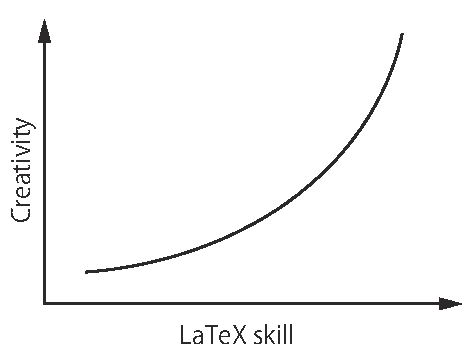
\includegraphics[scale = 1.0]{fig/sample.pdf}
  \caption{figure caption here.}
  \label{fig:sample}
\end{figure}

表は{\tt tabue}環境を使って作成します.表番号はTable~\ref{tab:sample}のように英語になります.位置指定は特になくても構いませんが,{\tt [t]}を使うと上部に配置されます.{\tt [h]}はやめましょう.
\begin{table}[]
  \caption{Table caption here.}
  \label{tab:sample}
  \centering
  \begin{tabular}{c|c|c}
    \textbf{Column 1} & \textbf{Column 2} & \textbf{Column 3} \\
    \hline
    Row 1, Cell 1 & Row 1, Cell 2 & Row 1, Cell 3 \\
    Row 2, Cell 1 & Row 2, Cell 2 & Row 2, Cell 3 \\
    Row 3, Cell 1 & Row 3, Cell 2 & Row 3, Cell 3 \\
  \end{tabular}  
\end{table}

\section{References}
参考文献は{\tt \textbackslash cite}を使って引用します\cite{kamimura22,Kamimura2022ASCC}.
参考文献リストはbibtexを使って自動生成します.
bibtexファイルはMendeleyやPaperpileなどのソフトウェアを使うとすぐに作れます.
bibtexの編集はVScodeでやってもいいですが,JavRefというフリーソフトがGUIが充実していて便利です.
書式は同梱のIEEEtranを使います.日本語文献の挿入は苦手かも.

\section{Build}
このテンプレートはlatexmkを使ってビルドすることをおすすめします.
設定は同梱のlatexmkrcファイルに記入されています.
bibtex周りも一気に自動でやってくれます.
ptex2pdfでもビルドできますが,latexmkの方が無駄が少なく高速です.

\section*{Acknowledgement}
研究費など,謝辞を忘れずに書いてください.

% \clearpage
\small
\bibliographystyle{IEEEtran} %IEEEtran.bstを参照
\bibliography{bibtexsample} % bibtexsample.bibを参照
\normalsize

\end{document}
